
\section{Discussion}
\label{sec:discussion}

The results in Section~\ref{sec:results} provide empirical evidence that tool routing can indeed be decomposed into semantic reasoning over entity types and compositional reasoning over a typed graph.
We now interpret what this decomposition means and where it applies.

\paragraph{Why does the decomposition help?}

The improvements arise from three complementary mechanisms.
First, the LLM's prediction target shifts from the tool catalog to a smaller entity type space, which graph reachability further constrains by 56--87\%.
Second, graph search constrains outputs to compositionally valid paths, exposing only 1.4--2.0 candidate tools per query instead of the full registry.
Third, every returned workflow is structurally valid by construction, eliminating hallucinated tool invocations entirely.
These reductions are determined by graph topology and apply independently of the LLM used for type prediction.

The magnitude of improvement is predictable from graph topology.
The tool-to-type ratio $|T|/|E|$ quantifies how much the decomposition compresses the selection problem: AAP has a 21:1 ratio (1,060 tools, 50 types) while Stripe has 3:1 (536 tools, 163 types).
On AAP, where the ratio is highest, Gemini 2.5 Flash improves from F1 = 0.29 (function calling) to 0.81 (few-shot TCR)---a nearly 3$\times$ gain.
On Stripe, where the ratio is lower and the type space is larger, the same model improves from 0.44 to 0.79.
The decomposition helps more when many tools collapse into few types, and this effect is amplified for less capable models: the Flash baseline-to-TCR gap is wider than the Pro gap on both domains.

\paragraph{Why multi-hop benefits most.}

To correctly route a $k$-hop query, direct selection must predict $k$ tools in the correct order, with each output type matching the next input type---errors compound at each step.
Under TCR, the model's task is invariant to chain length: it predicts two entity types regardless of whether the chain involves one hop or five, and graph search recovers intermediate tools the user never mentioned.
For example, ``get the logs for pods in production'' requires three tools (\texttt{list\_namespaces} $\rightarrow$ \texttt{list\_pods} $\rightarrow$ \texttt{get\_pod\_logs}), but the user refers only to the chain endpoints (\texttt{Namespace}, \texttt{PodLogs}).
This constant-complexity prediction is why multi-hop queries show the largest gap between TCR and direct selection.

\paragraph{Does the decomposition present a more tractable task?}

Across all model--domain combinations, LLMs correctly predict both entity types in 61\% of cases, compared to only 12\% where direct tool selection achieves perfect results (F1 = 1.0).
Although the two metrics are not directly comparable, the consistently higher accuracy supports the interpretation that the decomposed formulation presents a more tractable task.
Users naturally describe domain objects (``pods'', ``payments'', ``credentials'') rather than implementation mechanisms (\texttt{list\_pods}, \texttt{GetPaymentIntents}, \texttt{credentials\_list}); entity type prediction aligns with how queries are already phrased.

\paragraph{What is the error profile?}

The decomposition shifts errors from false positives to false negatives: TCR eliminates hallucinated tools and invalid compositions; remaining errors arise only from incorrect type predictions.
Average precision increases from 0.48 to 0.88 (+83\%), while recall increases from 0.67 to 0.83.
In safety-critical domains, returning no result is preferable to invoking incorrect tools.

\paragraph{Two-layer evaluation.}

Typed Composition Routing separates tool routing into two layers.
The first layer is entity-level routing: the model predicts source and target entity types, and the graph restricts the search space to tools that validly connect those types.
This layer does not claim to fully resolve user intent; it identifies the graph-valid candidate frontier.
The second layer is intent-level selection: choosing the specific tool or action among those candidates, such as selecting \texttt{list\_projects} rather than \texttt{create\_project} when the user asks to inspect existing projects.

This distinction matters for evaluation.
A prediction may be graph-valid even when it differs from the single reference tool annotation.
In such cases, the current intent-level F1 can understate the routing quality by penalizing valid alternate tools that connect the same entity pair.
We therefore report graph-valid metrics alongside the existing intent-level metrics.
Graph-valid precision measures whether predicted tools belong to the candidate set induced by the ground-truth entity pair, while intent F1 continues to measure whether the prediction matches the specific annotated tool answer.

\paragraph{Distinction from hierarchical routing.}

A natural objection is that TCR is simply hierarchical tool selection under a different name---first narrow the candidate set, then pick tools from it.
The distinction is deeper than the topology.
Hierarchical methods still predict \emph{tools} at every level: they cluster tools into categories and route the query through successively finer-grained tool subsets \cite{qin2024toolllm, li2025toolscope}.
The LLM's prediction target remains a tool at every stage; the hierarchy only reduces how many tools it must consider at once.
TCR changes the prediction target itself: the LLM predicts \emph{entity types}, and the graph generates the set of structurally valid tool chains---no tool name ever appears in the LLM's output.
This shift is what enables the structural guarantees---compositional validity, zero hallucination, analytically decomposable recall---that hierarchical selection cannot provide.
When multiple valid chains exist for the same entity pair, intent-level selection among guaranteed-valid candidates remains, but even this residual selection is constrained to a small set (typically 2--3 tools) that the graph has already verified for compositional correctness.

\paragraph{Relationship to retrieval-based selection.}

Retrieval-augmented tool selection ranks tools by embedding similarity to the query, reducing the candidate set before the LLM selects.
This is complementary to TCR rather than a direct alternative: retrieval ranks individual tools by semantic similarity, while composed queries require multi-step chains whose intermediate tools may have no lexical overlap with the query.
For instance, ``what is the last ARM artifact in the latest production drop'' has high similarity to an artifact-retrieval tool, but the prerequisite steps (listing drops, selecting a build) rank low precisely because the query does not mention them---they are structurally necessary but semantically invisible.
Retrieval-based filtering can thus eliminate tools that a valid composition requires.
TCR avoids this failure mode: graph search recovers the full chain from entity types, including intermediate tools the user never mentioned.
Retrieval could then serve as a reranker within the candidate set that graph search produces.

\paragraph{Asymmetric comparison with function calling.}

Native function calling benefits from model-level fine-tuning on large tool-calling corpora, making direct selection a \emph{trained} capability; entity type prediction under TCR is performed zero-shot via prompting.
Despite this asymmetry, TCR outperforms function calling across all model--domain combinations.

The recall decomposition (Eq.~\ref{eq:recall-decomposition}) makes the improvement path explicit.
When graph reachability is high ($R_c \approx 1.0$), end-to-end recall reduces to $\text{Recall} \approx P(\text{types correct})$: type prediction accuracy directly determines routing performance.
A domain-specific classifier fine-tuned over $|E|$ entity types faces a strictly smaller classification problem than a tool selector choosing among $|T|$ tools ($|E| < |T|$ in all evaluated domains).
This suggests that a fine-tuned type predictor---whether a small encoder model or a prompted LLM with in-context examples---could close the remaining accuracy gap while preserving the structural guarantees of graph search.

Figure~\ref{fig:improvement-path} quantifies this trajectory: precision is already high and stable ($r = 0.60$, graph constraint); recall is the bottleneck ($r = 0.59$), tracking type prediction accuracy directly; F1 shows the strongest correlation ($r = 0.72$, $p < 0.001$).
Since type prediction is classification over $|E|$ types (not $|T|$ tools), it is amenable to supervised training with modest annotation effort.
A natural follow-up is whether the semantic component must be performed by a large language model at all.

\begin{figure*}[t]
\centering
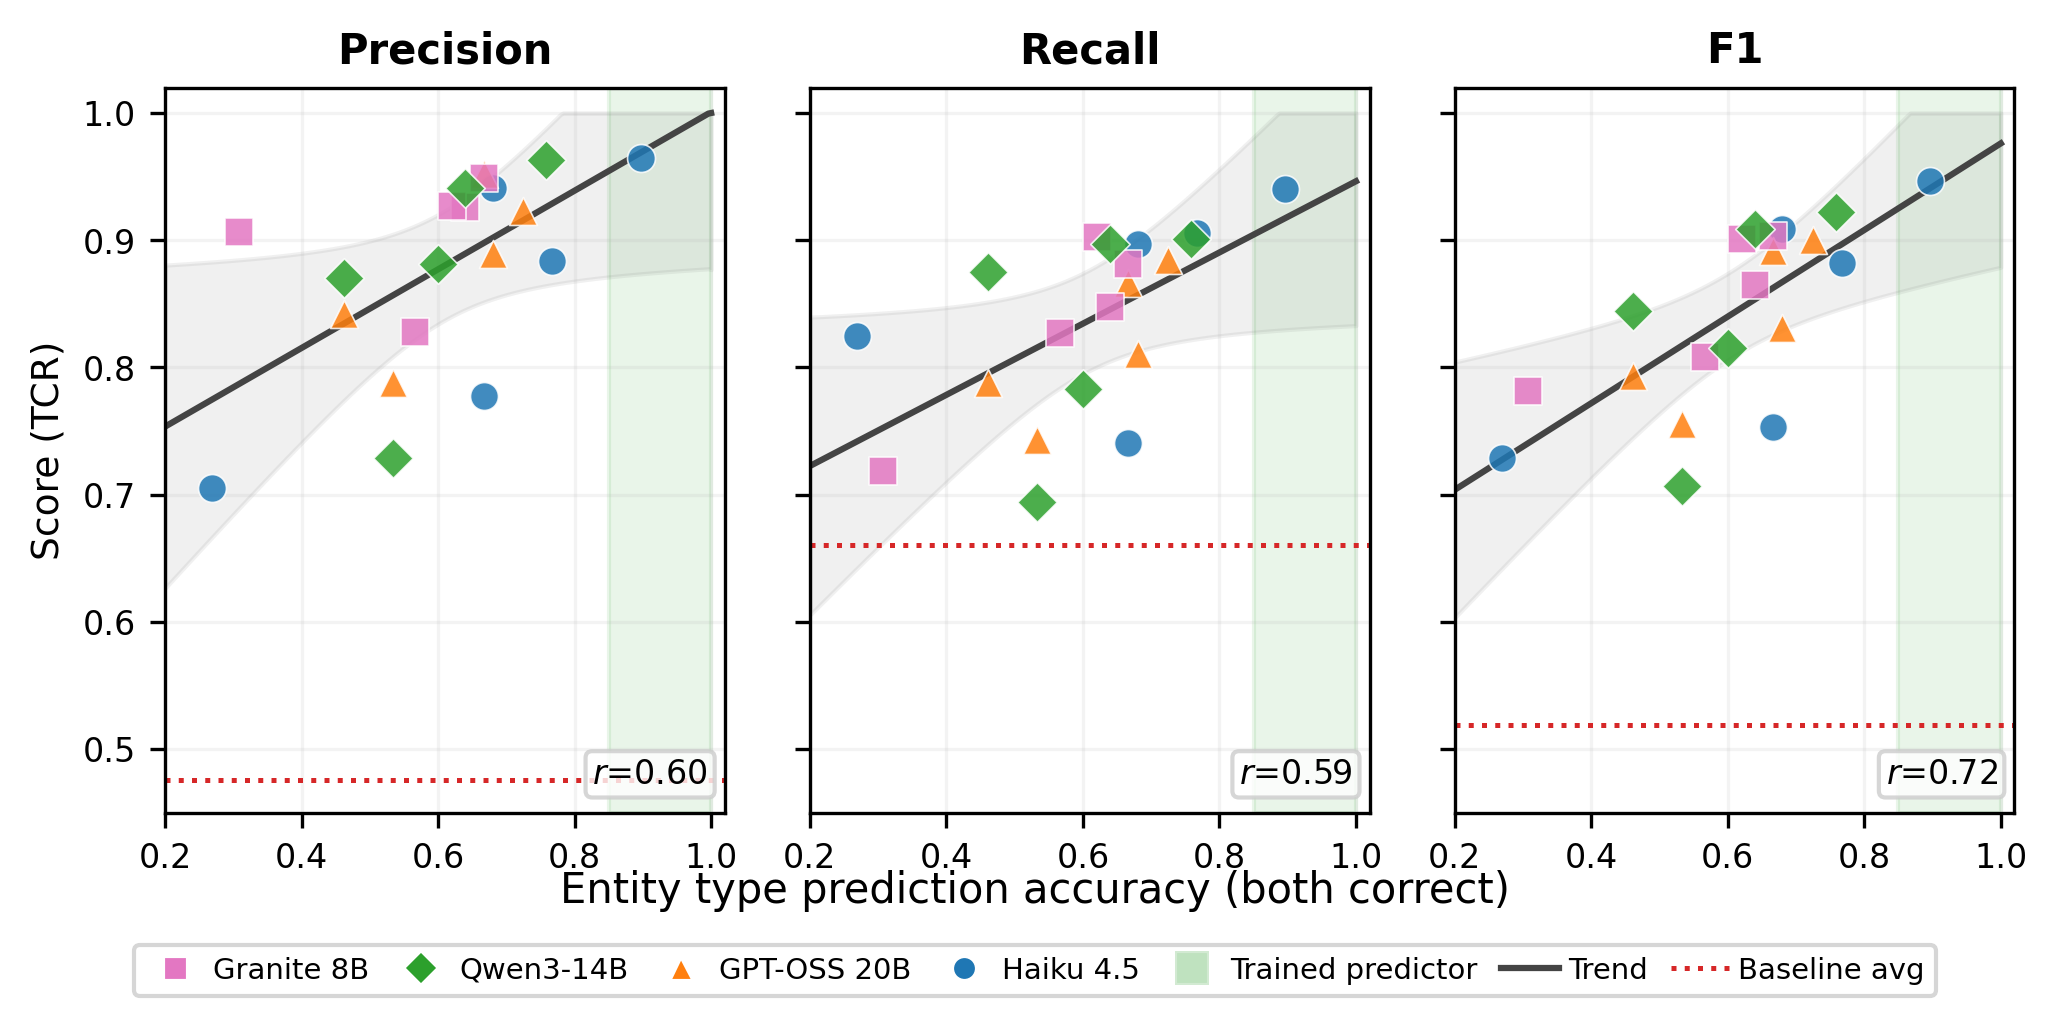
\includegraphics[width=\textwidth]{figures/improvement_path.pdf}
\caption{Entity type prediction accuracy vs.\ precision, recall, and F1 across 20 model--domain combinations. All TCR points (zero-shot type prediction) exceed the average baseline (red dotted lines), which uses models fine-tuned for tool selection. Precision is already high and stable (graph constraint); recall is the primary bottleneck, tracking type prediction accuracy. Green regions indicate the range accessible to a fine-tuned type predictor with higher accuracy.}
\label{fig:improvement-path}
\end{figure*}

\paragraph{Can the semantic component be replaced?}

To answer this, we train domain-specific type predictors on Stripe (536 tools, 163 types)\footnote{Stripe encoder: \url{https://github.com/jangel97/stripe-type-predictor}} and AAP (1,060 tools, 50 types)\footnote{AAP encoder: \url{https://github.com/jangel97/aap-type-predictor}}.
Each uses a frozen sentence encoder (all-mpnet-base-v2) with a shared hidden layer and two classification heads ($\sim$281K and $\sim$475K trainable parameters respectively), trained on synthetic examples with all test queries held out.
We also evaluate Gemini 2.5 Pro with \textbf{few-shot TCR} (10 in-context examples plus key rules in the system prompt) for comparison.

On AAP (Section~\ref{sec:production-eval}), the encoder achieves 96.3\% candidate recall vs.\ Gemini 2.5 Pro's 91.2\% with few-shot and 80.0\% zero-shot.
Few-shot prompting closes a large part of the gap---fixing ``list all X'' $\rightarrow$ Platform source routing and self-loop confusion---but the encoder retains its advantage on ambiguous (0.93 vs.\ 0.67) and multipath (0.93 vs.\ 0.73) queries, where domain-specific training provides structural understanding that in-context examples cannot fully convey.

Interestingly, Gemini 2.5 Pro with few-shot achieves higher \emph{exact type match} (91\% vs.\ 88\%) despite lower candidate recall.
This reflects higher source accuracy (97\% vs.\ 90\%): Gemini better identifies Platform as the root source for ``list all'' queries.
However, the encoder's higher target accuracy (97\% vs.\ 92\%) translates to better graph search outcomes, since an incorrect target sends BFS down the wrong path entirely, while source errors are sometimes recoverable through alternate graph edges.

Few-shot prompting scales differently across model sizes.
Granite 4.1 8B improves from 0.42 to 0.65 candidate recall with the same 10 examples---a larger absolute gain (+0.24) than Gemini (+0.11)---mainly from learning the Platform source pattern (source accuracy 57\%$\rightarrow$81\%).
However, its ceiling remains far lower: synonym (0.40) and multipath (0.47) recall stay weak because the 8B model lacks the capacity to map diverse terminology to entity types.
A crossover point emerges: Granite 0-shot performs \emph{better} with direct selection (F1\,=\,0.59) than with TCR (0.42 recall), but with few-shot TCR pulls ahead (0.65\,$>$\,0.59).
This suggests that the type abstraction helps only when the predictor exceeds ${\sim}$60\% exact match; below that threshold, keyword matching against tool descriptions outperforms incorrect type routing.

The largest gains come from the decomposition itself, not the choice of predictor.
The encoder achieves 0.96 candidate recall without requiring an LLM at inference time, at 6.8\,ms latency---three orders of magnitude faster than LLM-based prediction.

This validates the recall decomposition's prediction: a trained type predictor closes the remaining accuracy gap while preserving the structural guarantees of graph search, demonstrating that tool routing need not depend on frontier models.

\paragraph{Limitations.}

The formulation assumes tools can be modeled as typed transformations between entity types, which holds for typed API ecosystems but is less natural for imperative operations without typed outputs.
The current graph models unary transformations and sequential workflows only; multi-input dependencies, branching, and parallel composition would require extensions.
The composition graph must be constructed and maintained as tools evolve---Section~\ref{sec:production-eval} demonstrates automatic derivation from OpenAPI specifications, but generalization to arbitrary API surfaces remains open.
When multiple tools share the same type signature (e.g., \texttt{list\_projects} and \texttt{create\_project} both connect the same entity pair), the graph returns all of them as candidates; distinguishing among these requires intent-level reasoning that the graph does not provide.
Refining entity types to encode action semantics (e.g., separating read from write operations) could reduce such false positives, but at the cost of expanding the type space the model must predict over---the optimal granularity is domain-dependent.
The evaluation focuses on single-intent queries; compound requests would require an intent decomposition stage before graph search.

\paragraph{Broader pattern and future work.}

The decomposition instantiates a broader design pattern: mapping natural language to a structured intermediate representation that a deterministic solver can act upon, rather than asking the LLM to directly produce a final action sequence.
The contribution here is identifying entity types as the appropriate representation for tool routing, which explains why TCR generalizes across language models.
Promising extensions include weighted graph search, automatic graph construction from diverse API formats, support for non-linear composition, and integration with learned retrieval.
